%!TEX TS-program = pdflatex
%!TeX encoding = UTF-8
%!TeX spellcheck = en_US
%!TeX root = userManual.tex
%!TeX author = Dr.Ing. Mohammed Nour Abdelgwad Ahmed
%!TeX version = 1.5
%!TeX date = 2017.03.10

\documentclass[%
DIV=12,
abstract=on
%a5paper,                 % alle weiteren Papierformat einstellbar
%landscape,              % Querformat
%10pt,                       % Schriftgröße (12pt, 11pt (Standard))
%BCOR1cm,               % Bindekorrektur, bspw. 1 cm
%DIVcalc,                  % führt die Satzspiegelberechnung neu aus scrguide s.2.4
%twoside,                 % Doppelseiten
%twocolumn,            % zweispaltiger Satz
%halfparskip*,           % Absatzformatierung s. scrguide 3.1
%headsepline,           % Trennline zum Seitenkopf
%footsepline,            % Trennline zum Seitenfuß
%titlepage,                % Titelei auf eigener Seite
%normalheadings ,    % Überschriften etwas kleiner (smallheadings)
%idxtotoc,                 % Index im Inhaltsverzeichnis
%liststotoc,               % Abb.- und Tab.verzeichnis im Inhalt
%bibtotoc,                 % Literaturverzeichnis im Inhalt
%abstracton,              % Überschrift über der Zusammenfassung an
%leqno,                      % Nummerierung von Gleichungen links
%fleqn,                       % Ausgabe von Gleichungen linksbündig
%draft                        % überlangen Zeilen in Ausgabe gekennzeichnet
]
{scrartcl} %scrreprt

% Deutsche Anpassungen %
%\usepackage[ngerman]{babel}
\usepackage[T1]{fontenc}
\usepackage[utf8]{inputenc}
\usepackage{lmodern} 	%Type1-Schriftart für nicht-englische Texte
\usepackage{amssymb} %provides various useful mathematical symbols
\usepackage{amsthm}  %provides extended theorem environments
\usepackage{amsmath} %provides the align environment
\usepackage{xcolor}
\usepackage[bookmarks,
  bookmarksopen=false,
  bookmarksnumbered=true,
  pdftex,pdfhighlight=/N,
  linkcolor=blue!60!black,
  urlcolor=blue!60!black,
  colorlinks=true,
  citecolor=green!20!black,
  pdftitle={Steering Control for Autonomous Path Tracking},
  pdfsubject={EO2 Path Following Documentation},  % insert subtitle
  pdfkeywords={terramechanics, testbed, force measurement, soil contact interactions, impedance control, legged robots, simulation},
  pdfauthor={Dr.Ing. Mohammed Nour Abdelgwad Ahmed}]{hyperref}

% Packages für Grafiken & Abbildungen %
\usepackage{graphicx} 	%Zum Laden von Grafiken
%\usepackage{subfig} 	%Teilabbildungen in einer Abbildung
\usepackage{wrapfig}

% Bibliographiestil %
%\usepackage{natbib}

%------------------------------------------------------------------------------
\usepackage[automark,headsepline]{scrlayer-scrpage}
\clearpairofpagestyles
\cfoot[\pagemark]{\pagemark}
\lehead{\headmark}
\rohead{\headmark}
\pagestyle{scrheadings}

%\setkomafont{pagehead}{\normalfont\bfseries}
%\renewcommand*\pagemark{{\usekomafont{pagenumber}Page\nobreakspace\thepage}}
%\addtokomafont{pageheadfoot}{\upshape}
%------------------------------------------------------------------------------


  \usepackage{tikz} %for the revision No. block on the margin of title (first) page
%\usetikzlibrary{shapes}

\definecolor{thegrey} {gray}{0.5}
\definecolor{theshade}{gray}{0.94}
\definecolor{theframe}{gray}{0.75}

\usepackage{myboxedtheorem}
%\newboxedtheorem[options]{theo}{Theorem}{thCounter}
%boxcolor = black, titleboxcolor = black, background = white, titlebackground = white, titlecolor = black, thcounter=, size = .9\textwidth
%\newboxedtheorem[boxcolor=blue!20, background=blue!5, titlebackground=blue!20, titleboxcolor = blue!20]{theo}{Theorem}{anything}
\newboxedtheorem[boxcolor=theframe, background=theshade, titlebackground=thegrey,%
                 titlecolor = white, titleboxcolor = thegrey, size = 0.8\textwidth]{myColoredBox}{}{}

\newboxedtheorem[boxcolor=pink, titleboxcolor = pink, titlebackground=red!20, background=red!5]{mytheo}{}{}
%------------------------------------------------------------------------------
\setkomafont{title}{\normalfont\bfseries\small} %to set the tile font (I hate the default one ;))

\graphicspath{{./figures/}}
\pagestyle{empty} %Keine Kopf-/Fusszeilen auf den ersten Seiten.
%==============================================================================
%==============================================================================

\begin{document}
\thispagestyle{scrplain}

% title page ------------------------------------------------------------------
%\titlehead{Titelkopf}
\subject{ZuKa Documentation}
\title{Application of Industrial Robotic Arm in 3--Dimensional Milling (ZuKa)}
\subtitle{Steering Control for Autonomous Path Tracking}
\author{Dr.Ing. Mohammed Nour\footnote{corresponding author: Zagazig University, Faculty of Engineering, Computer and Systems Dept., Zagazig, Egypt, \href{mailto:mnahmed@eng.zu.edu.eg}{mnahmed@eng.zu.edu.eg}} %{Mohammed Ahmed}
\and{Ahmad Saeed}
\and{Ahmed Emam}
\and{Dua’a Samir}
\and{Donna Mustafa}
\and{Hoda Mahmoud}
\and{Reeham M. Ibrahim}
}

%\thanks{last revision \today}           % entspr. \footnote im Fließtext
\date{}%\today}                                 % in case another date other than today is wanted

\publishers{\vspace{15 mm}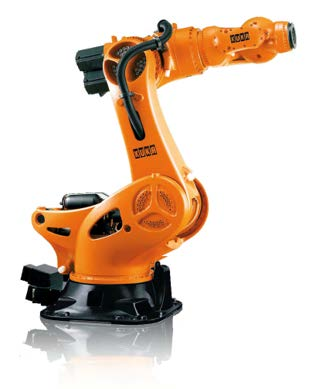
\includegraphics[width=0.55\textwidth]{kuka}}

% dedication ------------------------------------------------------------------
%\dedication{Widmung}

\maketitle      % show the title page

% add the revison side block
\begin{tikzpicture}[overlay,remember picture]
  \node[fill=black!30,text=white, inner ysep=2pt, inner xsep=20pt, rectangle,rotate=90]
    at ([xshift=10mm,yshift=0mm]current page.west)
    {\footnotesize{last revision \today}};
\end{tikzpicture}
%==============================================================================
% abstract after title and befor table of contents 
\vfill
\begin{abstract}
This report presents the derivation, design, and implementation of the ZUKA project.
\end{abstract}

%==============================================================================
\clearpage
\pagestyle{scrheadings}
\tableofcontents
%\listoftables
%\listoffigures
%\newpage
\clearpage
%==============================================================================

% main content ----------------------------------------------------------------
\cleardoublepage
\part{KUKA.Sim Pro}        \cleardoublepage
\section{Overview}
KUKA.Sim Pro is used for the complete offline programming of KUKA robots. This product allows the analysis of cycle times and the generation of robot programs. It also enables a real-time connection to the virtual KUKA robot controller (KUKA.OfficeLite). KUKA.Sim Pro is additionally used for building parametric components and defining kinematic systems, which can also be used in KUKA.Sim Layout and KUKA.Sim Tech. KUKA.OfficeLite is included in the KUKA.Sim Pro package. CAD importers are available as an option. This requires a purchasable license for each import interface. 
\begin{figure}[h]
\centering
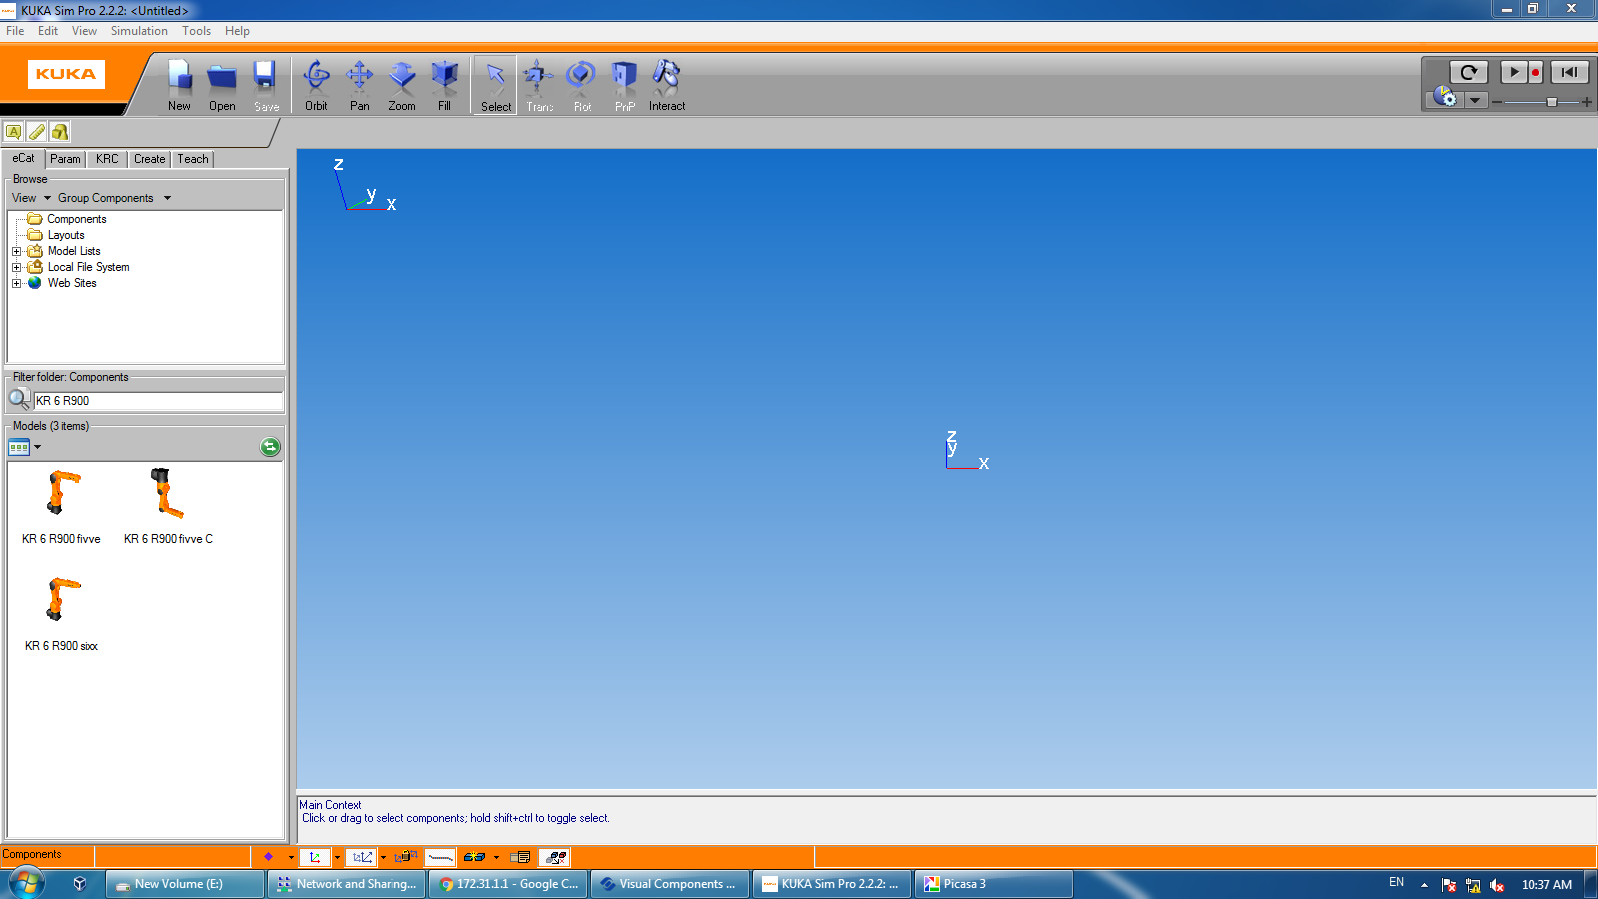
\includegraphics[width=0.9\textwidth]{figures/parts/33}
\label{fig:33}
\caption{KUKA.Sim Pro}
\end{figure}

\section{Requirements}
\begin{itemize}
	\item The minimum requirements for the computer are a 2 GHz CPU and 2 GB RAM, and an OpenGL capable graphics card with at least 512 MB RAM and a resolution of $1024 \times 768$ pixels or a similarly specified notebook.
	\item Supported operating systems are WIN XP - 32-bit or WIN 7 - 32/64-bit.
\end{itemize}

\section{Installaion}
Detailed installation steps can be found in the manual (KUKA.Sim 2.2 - Installation-en), starting page 9. 

\section{License Types}
There are different types of licensing for the KUKA software. License types are determined and verified in accordance with the purchase made from KUKA Roboter GmbH. 
The software licensing concerning the KUKA arm at Zagazig university is an educational bundle license. The serial number for the license is found in the booklet of the KUKA.Sim Pro CD. Information about different licensing bundles are obtained by contacting KUKA Roboter GmbH by email
\url{simulation@kuka-roboter.de.}
Further details about the steps of obtaining the serial key, for different commercial bundles,  are found on page 13 of (KUKA.Sim 2.2- Installation-en) manual.
\begin{mytheo}
 The serial number associated with this purchase is: \texttt {K5P22-N174H-AW7KY-9}
\end{mytheo}

\subsection{Stand-alone License}
The license is on the PC on which KUKA.Sim is used. The license key is then valid for this PC only. It can also be transferred to a different PC, but cannot be used on a two different PCs at the same time, or when either of the two PCs is off.

\subsection{Network License}
Network licenses provide a flexible way of using KUKA.Sim on more than one PC. When a license is requested by a PC, this license is then allocated to this PC. When KUKA.Sim is closed, the license becomes available again and can be accessed by other PCs. 
A license server is required to manage the network licenses. When KUKA.Sim Pro is started, the computer’s identity (IP address, please refer to \textbf {LAN connection} in manual Section “WorkVisual \& LAN connection”) is required occasionally, however, KUKA.Sim Pro needs to check with the local license server to make sure that KUKA.Sim Pro and server are on the same PC, which is required in the network license configuration.

\subsubsection{Installing the license server}
\begin{itemize}
\item Requirements:
“Microsoft Management Console” (MMC) must be installed on the license server. The software can be downloaded from the Microsoft website. In addition, “.NET framework 3.5” or higher should be installed. 
\end{itemize}
After following the installation steps, specified on page 17 of the \textbf {(KUKA.Sim
\textunderscore 2.2\textunderscore Installation\textunderscore en)}manual, there are a few steps required for activation of the serial number for the PC-Robot network.

For network licensing, an account linked with the purchase is created on the Visual Components website \url{http://www.visualcomponents.com/}. In the specified Customer portal \url{https://portal.visualcomponents.net/website/Login.aspx} sign in with the email \url{hodaeltahawy@gmail.com} and password \texttt{quails@123}.

In \textbf{My Products keys} tab, you will find the product key for KUKA.Sim Pro on the KUKA-PC device, at the Mechatronics lab. The license \textbf {is already activated} and will only require renewal after a period of 400 days starting 3-12-2016, which is on \textcolor{red}{7-1-2018}. 

\subsubsection{Manual Licensing}
Manual licensing is performed in case there was no internet connection available. All details about manual licensing in mentioned on page 21 of the (KUKA.Si\textunderscore 2.2
\textunderscore Installation\textunderscore en) manual. 

\textbf {Steps:}
\begin{enumerate}
\item Start the installation of KUKA.Sim Pro 
\item Enter the license key
\item Select “Activate manually” and save the request file
\item Go to the Visual components customer portal and use the given email and password, mentioned in the previous section, to login.
\item On the website, choose Manual Licensing, upload the request file and confirm.
\begin{figure}[h]
\centering
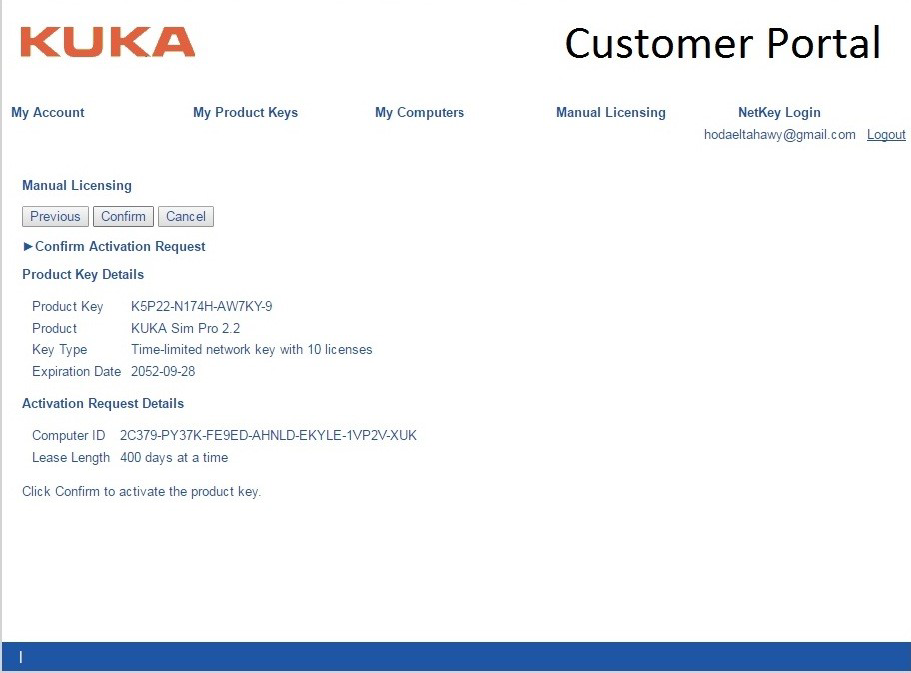
\includegraphics[width=0.9\textwidth]{figures/parts/44}
\label{fig:44}
\caption{Kuka Customer portal}
\end{figure}

\item The license should be activated
\item Download the license (.dat) file and click Finish. 
\item The license (.dat) file should be loaded into the license server, not the KUKA.Sim Pro interface, in order to complete the activation process.
\item After this process is completed, the network server interface should appear as shown in Figure.\ref{fig:55}
    \begin{figure}[h]
        \centering
        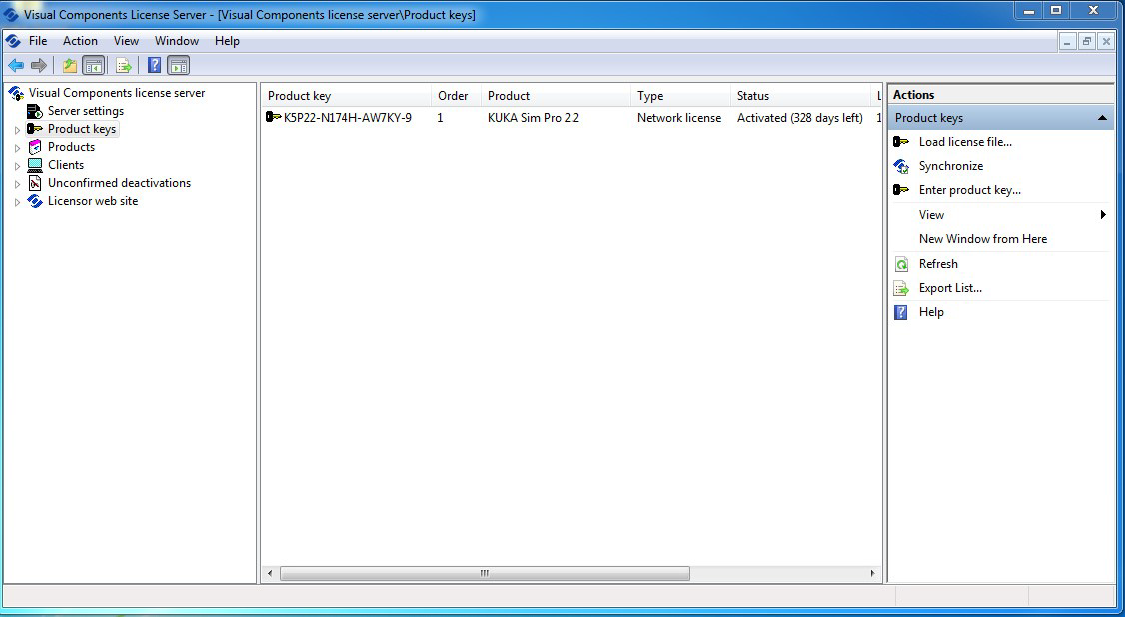
\includegraphics[width=0.9\textwidth]{figures/parts/55}
        \label{fig:55}
        \caption{Kuka network license server interface}
    \end{figure}
\end{enumerate} \cleardoublepage

\part {WorkVisual and LAN connection between KRC4 and the KUKA-PC}
\cleardoublepage
	\section{Introduction}
	The WorkVisual software package is the engineering environment for KR C4 controlled robotic cells. It offers the following functionalities:

	\begin{itemize}
		\item Configuring and connecting field buses
		\item Programming robots offline
		\item Configuring machine data
		\item Configuring RoboTeams offline
		\item Editing the safety configuration
		\item Transferring projects to the robot controller
		\item Loading projects from the robot controller
		\item Comparing a project with another project and accepting differences where necessary
		\item Managing long texts
		\item Managing option packages
		\item Diagnostic functionality
		\item Online display of system information about the robot controller
		\item Configuring traces, starting recordings, evaluating traces (with the oscilloscope)
		
	\end{itemize}

	\section{Hardware Requirements}
	Minimum requirements
	\begin{itemize}
		\item PC with Pentium IV processor, min. 1500 MHz
		\item 512 MB RAM
		\item DirectX8-compatible graphics card with a resolution of 1024x768 pixels
	\end{itemize}
	Recommended specifications
	\begin{itemize}
		\item PC with Pentium IV processor and 2500 MHz
		\item 1 GB RAM
		\item DirectX8-compatible graphics card with a resolution of 1280x1024 pixels
	\end{itemize}
	
	\section{Software Requirements}
	\begin{itemize}
		\item Windows 7 9Both the 32-bit version and the 64-bit version can be used)
		\item Or: Windows XP (32-bit version, with at least Service Pack 3, the 64-bit version cannot be used)
	\end{itemize}

	If the following software are not already installed on the PC, the installation wizard automatically starts their installation before preceding with the WorkVisual installation.
	\begin{itemize}
		\item .NET Framework 2.0, 3.0 and 3.5
		\item SQL Server Compact 3.5
		\item Visual C++ Runtime Libraries 
		\item WinPcap 
	\end{itemize}
\section{LAN connection}
In order to start file sharing process and to be able to use all functions of WorkVisual, a PC-Controller connection must be established. There are several ways to connect the KRC4 and KUKA-PC, one of which is setting up a local network for the connection of between several devices. This can be done by either setting static IPs for the connected devices and connecting them physically using a specified Ethernet cable, or by using a network router and assign dynamic IPs starting from a specified value, with specified number of connected devices. 
\subsection{To obtain and/or change IP values for the PC}
\begin{enumerate}
	\item Open "Network and sharing center" 
	\item Choose "Change adapter settings"
	\item Right click "Ethernet connections"
	\item  Choose "Internet protocol version 4 (TCP/IPv4)"
	\item  Choose "Properties"
	\item Next you either set static IPs or choose dynamic IPs to be set, in our case by the router.
\end{enumerate}

\begin{mytheo}[address ranges used]
   	The following address ranges are used by default by the
   robot controller for internal purposes. IP addresses from
   this range must not therefore be assigned by the user.
   \begin{itemize}
       \item 192.168.0.0 … 192.168.0.255
       \item 172.16.0.0 … 172.16.255.255
       \item 172.17.0.0 … 172.17.255.255
   \end{itemize}
\end{mytheo}

\subsection{LAN Configuration steps}
\begin{enumerate}
	\item Connect the PC and the KRC4 to the router using regular Ethernet cables.
	\item Access the router configuration page using the given data on the back of the router. (the router used in our case is TP-LINK, with username and password both being \textbf{admin})
	\item In the Interface setup change the LAN settings to your preferred values
	\item It is preferred to set the starting IP address similar to that of the KRC4 (172.31.147) to avoid conflicts. Network gateway value is (172.31.1.1) and subnet mask (255.255.0.0), all other settings shall remain unchanged.
\begin{figure}[h]
  \centering
  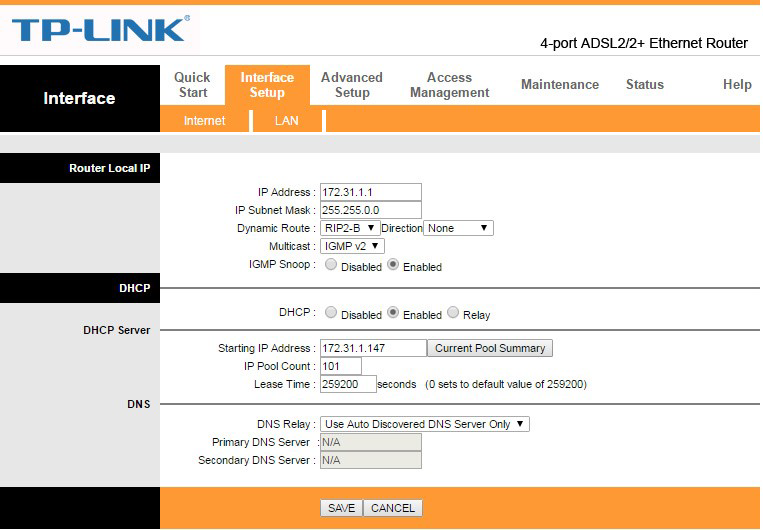
\includegraphics[width=0.9\textwidth]{figures/parts/11}
  \label{fig:11}
  \caption{Router LAN Configuration}
\end{figure}

	\item After changing these values, the IP address used to access the router settings will change from (192.168.1.1) to the set gateway value (172.31.1.1) but with the same user name and password.
\begin{figure}[h]
    \centering
    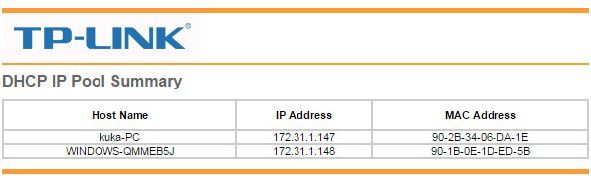
\includegraphics[width=0.9\textwidth]{figures/parts/12}
    \label{fig:12}
    \caption{IP address used to access the router settings }
\end{figure}

	\item The connection is now established and can be verified by checking the router LEDs
\end{enumerate}

%\section{Path Following Module }
%where $(x, y)$ represents the coordinates of the point $P$ located at mid-distance of the actuated wheels, the angle $\theta$ characterizes the vehicle chassis orientation, $\phi$ represents the vehicle steering \textbf{wheel} angle, and $L$ is the distance between the rear and front wheels axles.
%%------------------------------------------------------------------------------
%
%\subsection{Vehicle Model}
%For the vehicle, the kinematic model used (shown in Fig.\ref{fig:configurationVariables}) is:
%\begin{align}
%\dot{x} &= u_1 \cos\theta \notag\\
%\dot{y} &= u_1 \sin\theta \notag\\
%\dot{\theta} &=\frac{u_1 }{L} \tan\phi \notag\\
%\dot{\phi} &= u_2
%\label{eq:kinematicModel}
%\end{align}
%where $(x, y)$ represents the coordinates of the point $P$ located at mid-distance of the actuated wheels, the angle $\theta$ characterizes the vehicle chassis orientation, $\phi$ represents the vehicle steering wheel angle, and $L$ is the distance between the rear and front wheels axles.
%\begin{figure}[htbp]
%	\centering
%    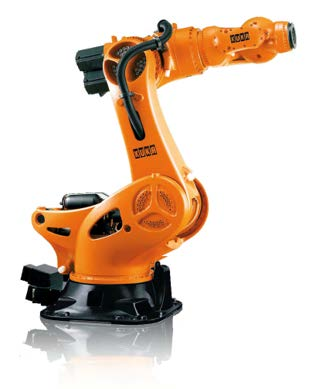
\includegraphics[width=0.4\textwidth]{kuka}
%    \caption{Configuration variables of the vehicle kinematic model}
%	\label{fig:configurationVariables}
%\end{figure}
%
% \begin{mytheo}[$\looparrowright$ Law of Large Numbers]
%    To calculate the horizontal position the kinematic differential equations are needed:
%    \begin{align}
%    \dot{n} &= u\cos\psi -v\sin\psi \\
%    \dot{e} &= u\sin\psi + v\cos\psi
%    \end{align}
%\end{mytheo}
%%==============================================================================
%
%\newpage
%\appendix
%\section{Appendix Part }
%where $(x, y)$ represents the coordinates of the point $P$ located at mid-distance of the actuated wheels, the angle $\theta$ characterizes the vehicle chassis orientation, $\phi$ represents the vehicle steering wheel angle, and $L$ is the distance between the rear and front wheels axles.
\end{document}
